
\chapter{Webová aplikace}

Tato kapitola popisuje zvolené postupy při psaní webové aplikace (backend a frontend).

Obrázek \ref{fig:structure_back} a obrázek \ref{fig:structure_front} popisují adresářové
struktury backendu a frontendu.
Některé méně důležite adresáře byly vynechány.
Seznam všech závislostí je uveden v souborech \textit{package.json} a \textit{package-lock.json}

\begin{figure} [!htb]
  \begin{itemize}
    \setlength\itemsep{.05em}
    \item \textbf{config} -- konfigurační soubory.
    \item \textbf{scripts} -- skripty pro vývoj.
    \item \textbf{test\_assets} -- obrázky pro testování rozpoznávání SPZ.
    \item \textbf{src} -- zdrojový kód.
    \begin{itemize}
      \setlength\itemsep{.05em}
      \item \textbf{apis} -- hepler funkce pro komunikaci s externím API pro rozpoznávání SPZ.
      \item \textbf{auth} -- autentifikace a autorizace.
      \item \textbf{cache} -- implementace mezipaměti.
      \item \textbf{db} -- připojení k databázi a nastavení GraphQL serveru Apollo.
      \item \textbf{endpoints} -- endpointy (ne GraphQL).
      \item \textbf{types} -- business logika aplikace, definice GraphQL schema, resolverů a mongoose modelů.
      \item \textbf{utils} -- datové struktury a ostatní helper funkce i pro testy.
    \end{itemize}
  \end{itemize}
  \caption{Adresářová struktura backendu.}
  \label{fig:structure_back}
  \end{figure}
  
\begin{figure}[!htb]
    \begin{itemize}
      \setlength\itemsep{.05em}
      \item \textbf{config} -- konfigurační soubory -- převzáno od CrazyFactory GmbH.
      \item \textbf{src/app} -- zdrojový kód.
      \begin{itemize}
        \setlength\itemsep{.05em}
        \item \textbf{apis} -- hepler funkce pro získávání obrázků z backendu.
        \item \textbf{components} -- komponenty uživatelského rozhraní.
        \item \textbf{constants} -- GraphQL dotazy, barvy, apod.
        \item \textbf{helpers} -- hepler funkce.
        \item \textbf{images} -- obrázky.
        \item \textbf{layouts} -- rozložení obrazovek.
        \item \textbf{pages} -- komponenty obrazovek.
        \item \textbf{redux} -- definice reducerů a stavů aplikace.
        \item \textbf{routes} -- definice cest obrazovek.
        \item \textbf{sagas} -- vedlejší efekty Redux akcí.
      \end{itemize}
    \end{itemize}
    \caption{Adresářová struktura frontendu.}
    \label{fig:structure_front}
  \end{figure}

\section{Obrazovky}

Dle požadavků z úvodu mějme po příhlášení do webového rozhraní následující obrazovky,
mezi kterými bude uživatel přepínat pomocí hlavního menu.
Snímky obrazovek lze vidět v sekci \ref{screens}.

\begin{itemize}
  \setlength\itemsep{.05em}
  \item \textbf{Zařízení} -- správa zařízení zachycujících fotografie SPZ, která lze autentifikovat do systému pomocí
        QR kódu.
  \item \textbf{Pravidla a Filtry} -- definice parkovacích pravidel a filtrů vozidel (popsáno v \ref{analysis_parking_schema}).
        Pro ověření půjde si parkovací pravidla a filtry odsimulovat.
  \item \textbf{Statistiky} -- detailněji zobrazené údaje o počtu parkování a výdělku podle roku, měsíce a dne s grafy.
  \item \textbf{Vozidla a Parkování} -- prohlížení vozidel a jejich parkování.
  \item \textbf{Správa účtu} -- změna údajů a hesla současně přihlášeného uživatele.
  % \item \textbf{Správa uživatelů} -- přidávání, odebírání a úprava uživatelů a jejich operávnění.
\end{itemize}

\section{GraphQL resolvery}

Protože GraphQL je primárním způsobem komunikace mezi frontendem a backendem, stojí za to si vysvětlit základní stavební bloky
GraphQL -- resolvery, které tvoří strom. Vzpoměňme si na příklad z předchozí kapitoly na obrázku \ref{fig:graphql_example}.
Zde kořenem stromu je resolver \textit{userSearch}, jenž přijímá argumenty potřebné pro jeho běh, ty jsou v tomto případě
povinné (ale nemusí). Kořenový resolver je funkce vracející nějaký typ, v tomto případě typ \textit{UserSearchResult}, který udává nalezené
uživatele (\textit{UserSearchResult.data}) a stránkování (v příkladu vynecháno).
Při návrhu tohoto resolveru bychom si mohli rozmyslet, že údaje o stránkování vynecháme a vrátíme pouze
pole nepřázdných uživatelů -- typ \textit{[User!]}.
Máme dva druhy typů: skaláry (listy stromu) a objekty (uzly stromu).
Typ \textit{User} je objekt a má v sobě také nějaké hodnoty a vrátí se nám jen ty, na které se zeptáme. Měl-li by typ \textit{User}
další objekty, mohli bychom se zeptat i na jejich hodnoty. Kdybychom psali aplikaci pro veterinární kliniku, mohli bychom se zeptat
třeba na jména mazlíčků.

Jak toto implementujeme? Pro každý kořenový resolver musíme napsat funkci, která buď přímo vrátí požadovaný objekt s atributy a nebo
k typu, který náš kořenový resolver vrací, napíšeme další resolvery, které vrací opět objekty, nebo skaláry.
Kdybychom se databáze ptali na uživatele i s
mazlíčky (v SQL terminologii bychom provedli JOIN), tak bychom nemuseli pro typ \textit{User} psát resolver pro mazlíčky, kde bychom
se dotázali na mazlíčky našeho uživatele.
\citep[viz][]{GraphQLDoc}

Zároveň můžeme provádět virtualizaci atributů -- přidávat atributy, které v databázi nemáme, ale pro webové rozhraní se hodí.
Hypotetickým příkladem budiž celková zaplacená částka zákazníkem, která se v případě potřeby vypočítá.

\subsection{Obecné resolvery}

Jelikož se většina operací nad modeli se opakuje, byli napsány obecné resolvery jako HOF (Higher-Order-Function)
pro vytváření, úpravu, mazání, vyhledávání a získávání modelů v relaci.
Měnící se část je pak pouze definice databázového modelu. Díky GraphQL nemusíme ani ověřovat datové typy, které dostaneme od klienta --
GraphQL toto udělá za nás díky schema, které tvoříme my.

\begin{figure}
\lstset
{ %Formatting for code in appendix
    basicstyle=\footnotesize,
    numbers=left,
    stepnumber=1,
    showstringspaces=false,
    tabsize=1,
    breaklines=true,
    breakatwhitespace=false,
}
\begin{lstlisting}
function gqlPopulate<D extends mongoose.Document,
                     K extends keyof D>(
  modelGetter: ModelGetter<D>,
  key: K
): Resolver {
  return async function(obj: D, args, ctx: Context, info) {
    const model = modelGetter(ctx);
    const keyStr = key.toString();
    if (obj.populated(keyStr)) {
      return obj[key];
    } else {
      const populated: D = await model.populate(obj, {
        path: keyStr
      });
      return populated[key];
    }
  };
}
\end{lstlisting}
\end{figure}

Zde lze vidět funkci vracející resolver, který vrátí objekt v relaci (provede JOIN v SQL terminologii),
pokud ho vlastnící objekt ještě nemá. Na sedmém řádku se získá model z funkce v \textit{lexical-scope} funkce
vracející resolver. Proměnná \textit{ctx} definuje kontext resolveru a obsahuje modely a klienta, aby
bylo snažší resolvery testovat -- jedná se o \textit{dependency-injection}.

Na šestém řádku lze vidět parametry, které dostává každý resolver. První parametr je objekt vrácený nadřazeným resolverem,
pokud nějaký je. Druhý parametr obsahuje klientem specifikované argumenty, například id hledaného uživatele.
Třetí parametr je již zmíněný kontext, jeho
obsah si ale definijeme samy v jiné části zdrojového kódu. Poslední parametr obsahuje info o dotazu samotném --
jaké parametry si klient vyžádal apod.

\section{Autentizace a autorizace} \label{auther_authen}

Autentifikace lidských uživatelů probíhá pomocí standardního hesla a zařízení pomocí dlouhého, náhodně generovaného hesla,
které je posíláno na frontend ve formě QR kódu, které zařízení naskenuje.
Po úspěšné autentizaci obdží klient token, který kdyby klient posílal v souboru Cookie,
tak bychom se vystavovali riziku útoku CSRF/XSRF.
Místo toho bude klient posílat token v hlavičce \textit{Authorization}.

Podle tokenu klienta jednoznačně identifikujeme a víme jeho oprávnění. Endpointy a GraphQL resolvery zabezpečíme tak,
že každý endpoint nebo resolver, který vyžaduje oprávnění, dáme jako argument HOF (Higher-Order-Function)
\textit{checkPermissions} společně s požadovanými oprávněními. \textit{checkPermissions} pak zavolá původní endpoint
nebo resolver pouze pokud má klient dostatečná oprávnění.

\section{Business logika}

\subsection{Parkovací pravidla} \label{analysis_parking_schema}

\begin{itemize}
  \setlength\itemsep{.05em}
  \item Různá vozidla mohou podléhat ruzným pravidlům.
  \item Pravidla mají prioritu.
  \item Pravidla mají časové omezení.
  \item V jednu chvíli může platit více pravidel.
\end{itemize}

Mechanismus, kterým umožníme vozidlům být ovlivněna některými pravidly,
budou filtry.
Pro dostatečnou flexibilitu je zapotřebí oddělit samotná pravidla od jejich
priority, časového intervalu platnosti i filtrů,
k čemuž bude sloužit objekt typu \texttt{ParkingRuleAssignment}.

% TODO - add a db schema image that takes less space
\begin{lstlisting}
type ParkingRuleAssignment {
  rules: [ParkingRule]!
  start: DateTime!
  end: DateTime!
  # ALL nebo NONE
  vehicleFilterMode: VehicleFilterMode!
  vehicleFilters: [VehicleFilter!]
  priority: NonNegativeInt!
}

type VehicleFilter {
  id: ID!
  name: String!
  action: VehicleFilterAction!
  vehicles: [Vehicle!]!
}
\end{lstlisting}

Filtrování bude mít dva módy: začneme se všemi vozidly (ALL) a začneme bez vozidel (NONE).
Následné filtry mohou buď přidávat, nebo odstraňovat jednotlivá vozidla.
Hodí se mít filtry uložené separátně, aby mohli být využity několikrát.

Pro zjednodušení algoritmů, uvalíme omezení: ve stejný čas nesmí existovat více \texttt{ParkingRuleAssignment}
se stejnou prioritou.

\subsubsection*{Algoritmus filtru vozidel}

\textit{Vstup: objekt \texttt{ParkingRuleAssignment}, vozidlo}

\textit{Výstup: boolean určující platnost}
\begin{enumerate}
  \setlength\itemsep{.05em}
  \item Na základě módu filtrování si budeme udržovat množinu buď odstraněných vozidel (mód ALL), nebo přidaných vozidel (mód NONE).
  \item Podle příslušné akce filtrů (odstranit nebo přidat) budeme množinu našich vozidel manipulovat. Např. je-li mód ALL a filtr odstraňuje, do množiny si vozidla přidáme.
  \item Pokud je vozidlo ve výsledné množině, tak pro něj \texttt{ParkingRuleAssignment} platí pokud je filtrovací mód NONE a neplatí pokud je mód ALL. Opačné výsledky nastanou, pokud vozidlo v množině není.
\end{enumerate}

Časová i paměťová složitost algoritmu je ${\cal O}(N)$, kde $N$ je počet filtrů.

Tento algoritmus lze potenciálně rozdělit na předvýpočet (kroky 1. a 2.) a ověření (krok 3.).
To je jedna možnost, která zvýší paměťovou náročnost, protože bychom si museli pamatovat množiny, což je nepraktické.
Je-li uživatel příčetný, počet použitých filtrů nebude obrovský, a tudíž je lepší zvolit následující způsob cachovaní.
Zapamatujeme si výsledky pro určitý seznam filtrů pro konkrétní vozidlo pouze při běhu algoritmu, který je
vysvětlen v následující kapitole, čímž následující algoritmus zrychlíme.

\subsubsection*{Algoritmus pro aplikaci ParkingRuleAssignmentů}

\begin{figure}[!htb] \centering
  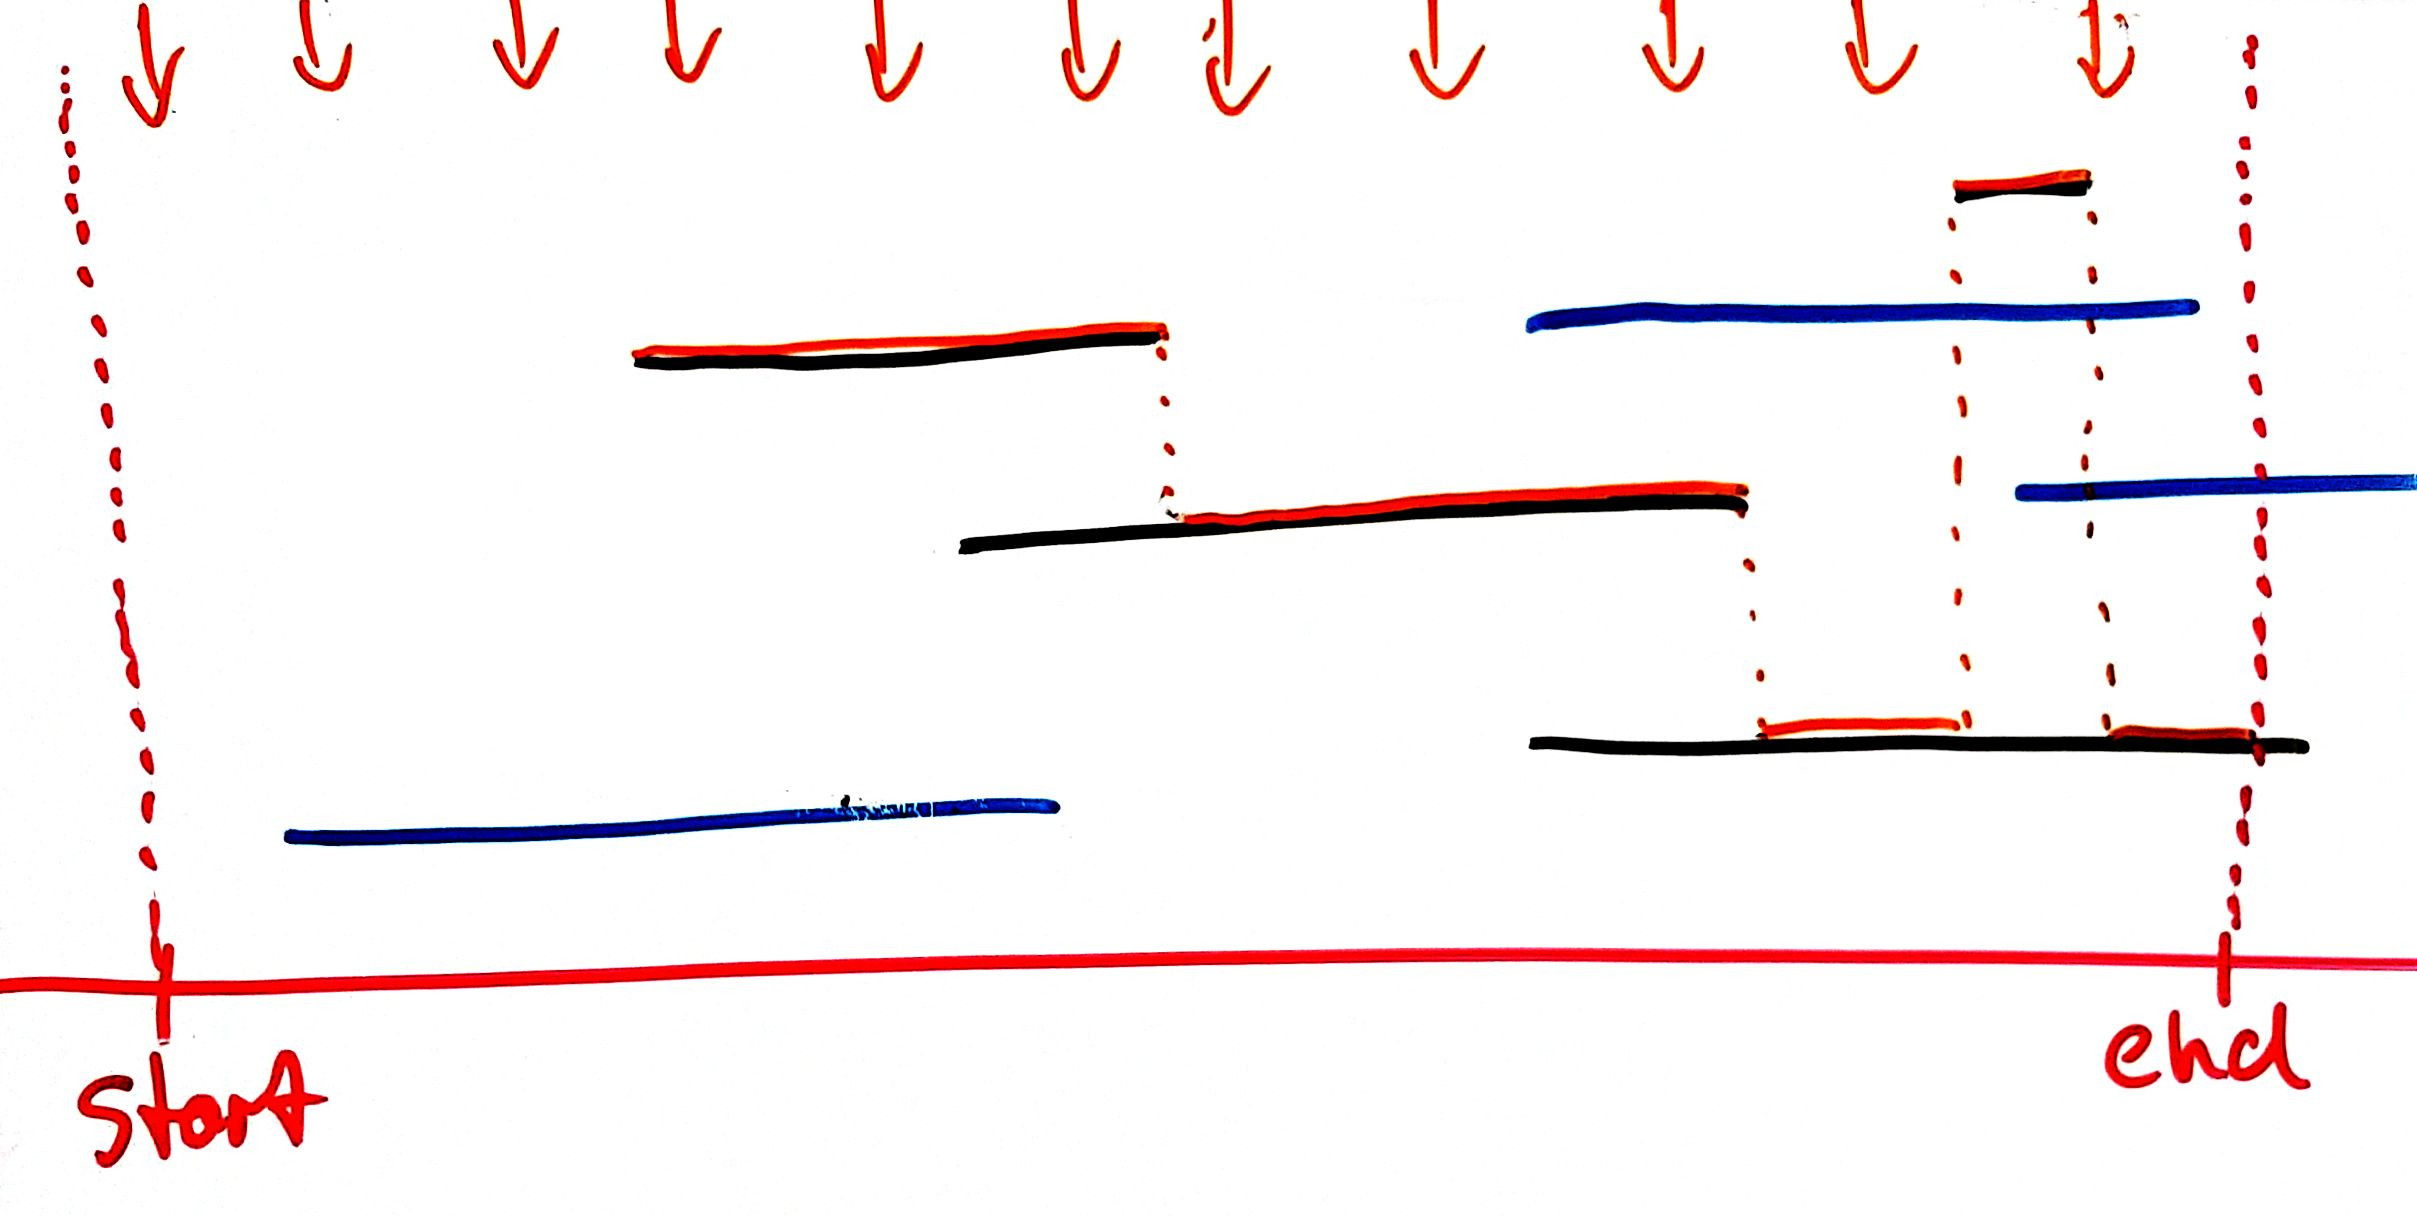
\includegraphics[width=145mm]{../img/rules_drawing.jpg}
  \textit{Modré úsečky neplatí kvůli filtrům nebo protože jsou deaktivované. Oranžová čára značí výstup požadovaného algoritmu.}
  \caption{Ilustrace problému úseček.}
  \label{fig:rules_drawing}
\end{figure}

V jednom čase může existovat více objektů typu \texttt{ParkingRuleAssignment} avšak s různou prioritou.
Může se stát, že aplikovaných \texttt{ParkingRuleAssignment} bude několik (různé priority, vyprší platnost, etc.).

Situaci si lze představit jako několik úseček navzájem rovnoběžných úseček v různých výškách, které se neprotínají.
Nás nyní zajímá, na které a v jakých intervalech na ně dopadne světlo, pokud na ně kolmo zeshora posvítíme.
Situaci lze vidět na obrázku \ref{fig:rules_drawing}.

Pro zjednodušení předpokládejme, že všechny \texttt{ParkingRuleAssignment}, které zpracováváme, platí pro naše vozidlo.
Přidat tuto kontrolu později je triviální.

\textit{Vstup: seznam \texttt{ParkingRuleAssignmentů} odpovídající pro interval pobytu vozidla na parkovišti, vozidlo}

\textit{Výstup: seznam \texttt{ParkingRuleAssignmentů} s časy platnosti}
\begin{enumerate}
  \setlength\itemsep{.05em}
  \item Seřadíme si začátky a konce úseček podle jejich času.
  \item Vytvoříme si haldu pro odkládání úseček, která řadí podle priority -- větší výše.
  \item Vytvoříme si seznam aplikovaných pravidel s časy (časy mohou se lišit od počátečních i koncových časů).
  \item Nechť \textit{s} je současná úsečka a \textit{$t_s$} čas zvolení \textit{s} (čas zvolení se může lišit od začátku úsečky).
  \item Pro každou událost \textit{u} značící začátek/konec úsečky (aplikaci pravidla) \textit{p}:
  \begin{enumerate}
    \item Pokud se jedná o začátek nové úsečky:
    \begin{enumerate}
      \item Pokud není zvolená úsečka:\\
            \textit{$t_s$} $\leftarrow$ \textit{p.start}\\
            \textit{s} $\leftarrow$ \textit{p}
      \item Pokud je zvolená úsečka a \textit{p} má vyšší prioritu než \textit{s}:\\
            \textit{s} dáme do seznamu aplikovaných pravidel se začátkem \textit{$t_s$} a koncem \textit{p.start}.\\
            \textit{s} dáme na haldu, pokud \textit{s.end} > \textit{p.end}.\\
            \textit{$t_s$} $\leftarrow$ \textit{p.start}\\
            \textit{s} $\leftarrow$ \textit{p}
      \item Pokud je zvolená úsečka a \textit{p} má nižší prioritu než \textit{s} a \textit{p.end} > \textit{s.end}:\\
            \textit{s} dáme na haldu
    \end{enumerate}
    \item Jinak (jedná se o konec nějaké úsečky):
    \begin{enumerate}
      \item Přidáme \textit{s} do seznamu aplikovaných pravidel se začátkem \textit{$t_s$} a koncem \textit{s.end}.
      \item Taháme z haldy, dokud nedostaneme úsečku s koncem později než konecm \textit{p}, nebo dokud halda není prázdná.
      \item Pokud jsme z haldy vhodnou úsečku vytáhli, použijeme ji. V opačném případě vyprázdníme \textit{s} a \textit{$t_s$}.
    \end{enumerate}
  \end{enumerate}
\end{enumerate}

Algoritmus zajisté doběhne, protože máme konečný počet událostí a v každém cyklu jednu zpracujeme.
Paměťová složitost je zřejmě lineární. Časová složitost bez filtrování je ${\cal O}(N\cdot{logN})$, kde $N$ je 
počet úseček, protože
využijeme některého z rychlích zaření a protože použijeme binární haldu a lepší. Počet operací nad haldou,
který by konečnou složitost mohl změnit, je naštestí lineární. Největší počet operací nad haldou dostaneme tak, že
každou přidanou úsečku umístíme tak, aby při zpracování jejího konce i začátku došlo k přidání a odebrání z haldy
(nejedná o tu samou úsečku). Jedna z takovýchto uspořádání je například pyramida, popřípadě zikkurat.
Tedy s každou přidanou úsečkou se počet operací nad haldou zvýší maximálně o $2$.

Přidáme-li filtrování, tak v nejhorším případě budeme ověřovat platnost každé úsečky. Bude-li $M$ průměrný počet
filtrů, pak je časová složitost ${\cal O}(N\cdot{M})$. 
% Při rozumném počtu \texttt{ParkingRuleAssignment} v daném intervalu je algoritmus velice rychlý

\section{Uživatelské rozhraní}

Jelikož autor neměl zkušenosti s vývojem webového uživatelského rozhraní, rozhodl se využít starter projekt
společnosti Crazy Factory, který pojí vybrané technologie dohromady a mandatuje projektu základní strukturu.
Navíc podporuje překlady, reportování chyb apod., což vytvářet z ničeho je obtížné. \citep[viz][]{CFProj}

\subsection{Redux a persistence stavu}

Jak již bylo zmíněno v předchozí kapitole, uživatelské rozhraní používá Redux pro sdílení stavu mezi komponentami.
Stav v Reduxu je strom, jenž je upravován akcemi. Akce a současný stav je předán takzvaným \textit{reducers}, což jsou prosté funkce,
které vrátí stav nový. \citep[viz][]{ReduxCore} Prostost reducerů umožňuje testovatelnost.

Jako příklad konkrétního využití budiž sdíleí některých údajů mezi obrazovkami.
Napřídklad sdílení vozidla mezi stránkou s vozidly a stránkou s pravidly, schopnost seznamu parkování zvolit vozidlo a mnoho dalších.

Některé komponenty jsou pak na stavu závislé a dojde k jejich překreslení, pokud se jimi čtený stav změní, což je též zařízeno
Reduxem. Jedná se vlastně o formu \textit{dependency-injection}. Stejným mechanismem jsou do komponent vkládány
funkce vyvtvářející akce a jiné vedlejší efekty, což dělá tyto komponenty snadno testovatelné.

K tomu abychom mohli uložit stav aplikace po zavření okna, použijeme knihovnu \textit{redux-persist}, která poskytuje
HOF funkci, které dáme reducer, a ona změny, které způsobí, někam uloží. \citep[viz][]{reduxpersist}
V našem případě se jedná o \textit{localstorage}.

\subsection{Typy komponent}

Níže je rozlišení komponent podle jejich interakce s ostatními a míry autonomie.
Jedná se o spektrum, ne o definitivní kategorie.

\begin{itemize}
  \setlength\itemsep{0.05em}
  \item \textbf{Bez vnitřního stavu} -- může se jednat o tlačítka, vstupy textu apod. Tyto komponenty jsou zcela řízeny
      nadřazenou komponentou.
  \begin{itemize}
    \setlength\itemsep{0.05em}
    \item \textbf{Strukturní} -- delegují data dalším komponentám a mohou mít podřízené komponenty. Příkladem budiž sekce třeba v 
        uživatelském rozhraní se stejným stylem.
  \end{itemize}
  \item \textbf{S vnitřním stavem} -- tyto komponenty údávají stav podřízeným komponentám.
  \begin{itemize}
    \setlength\itemsep{0.05em}
    \item \textbf{Napojené na Redux} -- jedná se o podtyp komponent s vnitřním stavem, které část stavu berou z Reduxu.
    \item \textbf{Komunikující se světem} --  komunikují s vnějším světem. Například posílají GraphQL dotaz backendu.
  \end{itemize}
\end{itemize}

\subsection{Grafy}

Grafy jsou potřeba na stránce se statistikami. K tomu byla použita knihovna \textit{react-google-charts},
což, jak název napovídá, je port knihovny \textit{google-charts} do Reactu. Ta kromě obvyklích grafů umí
například i takzvaný kalendářový graf, jenž lze vidět na obrázku \ref{fig:google_charts}.

\begin{figure}[!htb] \centering
  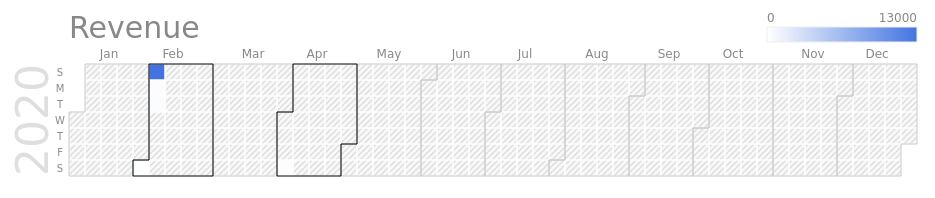
\includegraphics[width=145mm]{../img/google_charts.png}
  \caption{Kalendářový graf z knihovny react-google-charts.}
  \label{fig:google_charts}
\end{figure}


\subsection{Obecná vybírátka modelů}

Dle principu neopakování se bylo vytvořeno několik obecných UI komponent, které umožňují vyhledávání libovolných
modelů a jejich volbu a využití v ostatních komponentách. Ve zdrojovém kódu je implementujeme jako
HOF (Higher-Order-Function), což je funkce vracející další funkce -- konkrétní komponenty.
Měnící se části, které do těchto obecných komponent budeme vkládat je komponenta renderující jediný model
(\textit{renderModel}),
GraphQL dotaz pro získávání modelů (\textit{queryString}), funkce, jejímž vstupem je odpověď na GraphQL dotaz a výstupem je
samotné pole modelů (\textit{modelArrayGetter}), a funkce, jejímž vstupem je dotazovací řetězec a výstupem jsou
argumenty pro GraphQL dotaz (\textit{identifierToOptions}).

Obrázek \ref{fig:picker_lifecycle} ukazuje tok dat v jednom z obecných vybírátek.
Obrázek \ref{fig:picker_component} ukazuje vyrenderovanou komponentu vybírátka.

Další vybírátka abstrahují i vstup od uživatele, takže lze použít například kalendář.

\begin{figure}[!htb] \centering
  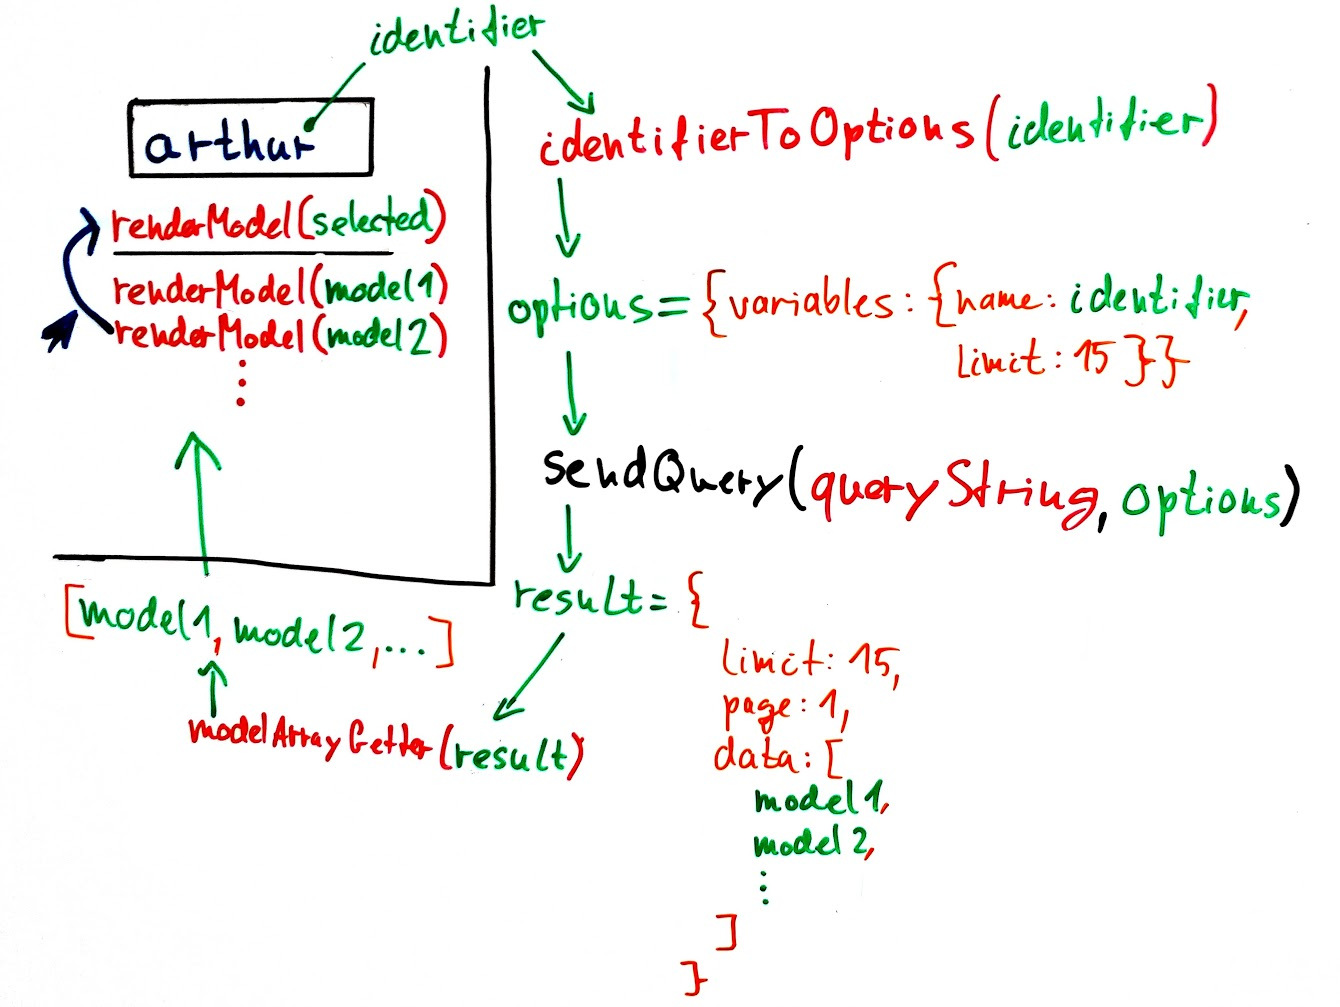
\includegraphics[width=145mm]{../img/picker_lifecycle.jpg}
  \caption{Tok dat v jednom z obecných vybírátek.}
  \label{fig:picker_lifecycle}
\end{figure}

\begin{figure}[!htb] \centering
  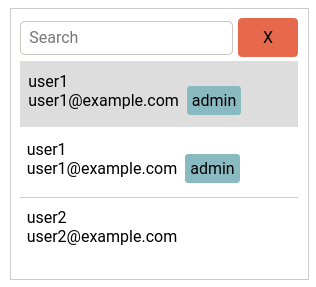
\includegraphics[width=70mm]{../img/picker_component.png}
  \caption{Vyrenderovaná komponenta jednoho vybírátka.}
  \label{fig:picker_component}
\end{figure}

% \newpage

\section{Snímky obrazovky obrazovek} \label{screens}

\subsection*{Zařízení}

\begin{figure}[!htb] \centering
  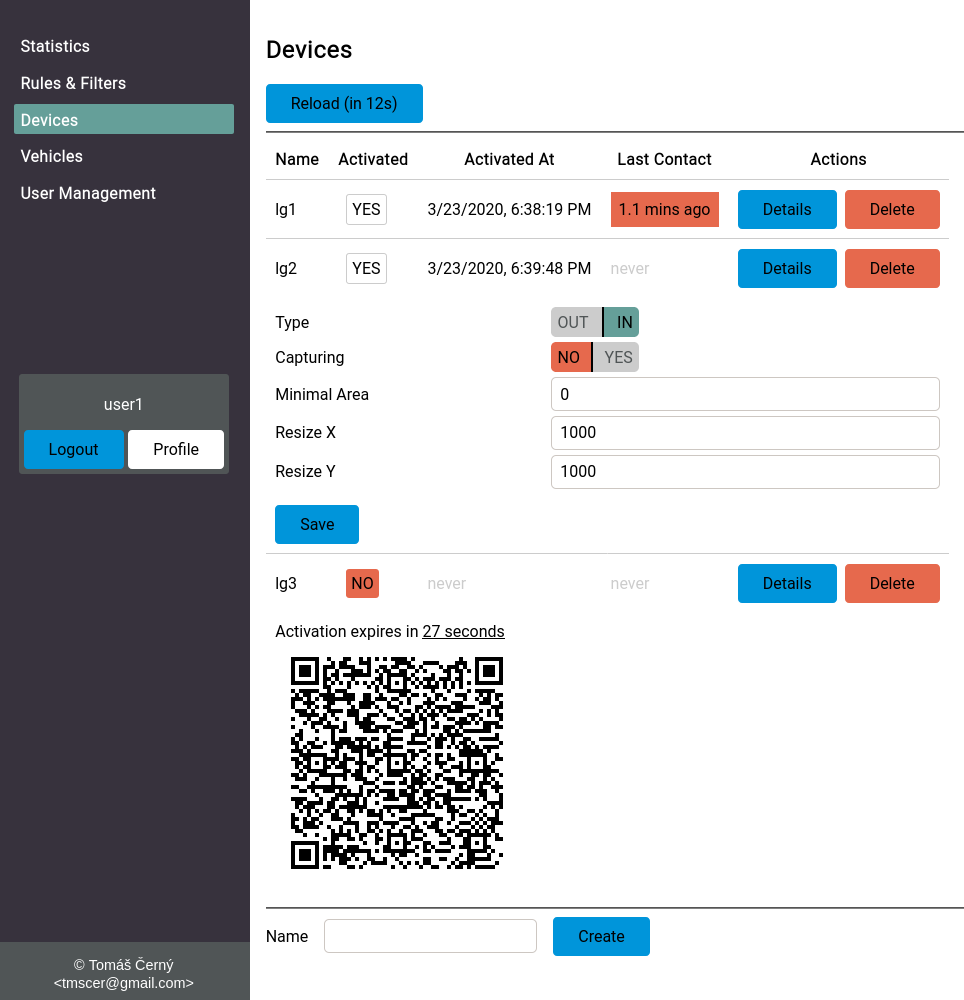
\includegraphics[width=145mm]{../img/page_devices.png}
  \caption{Stránka pro zařízení.}
  \label{fig:page_devices}
\end{figure}

Viz obrázek \ref{fig:page_devices}.
Po vypršení QR kódu je uživateli nabídnuto vytvořit nový.

\subsection*{Pravidla a Filtry}

\begin{figure}[!htb] \centering
  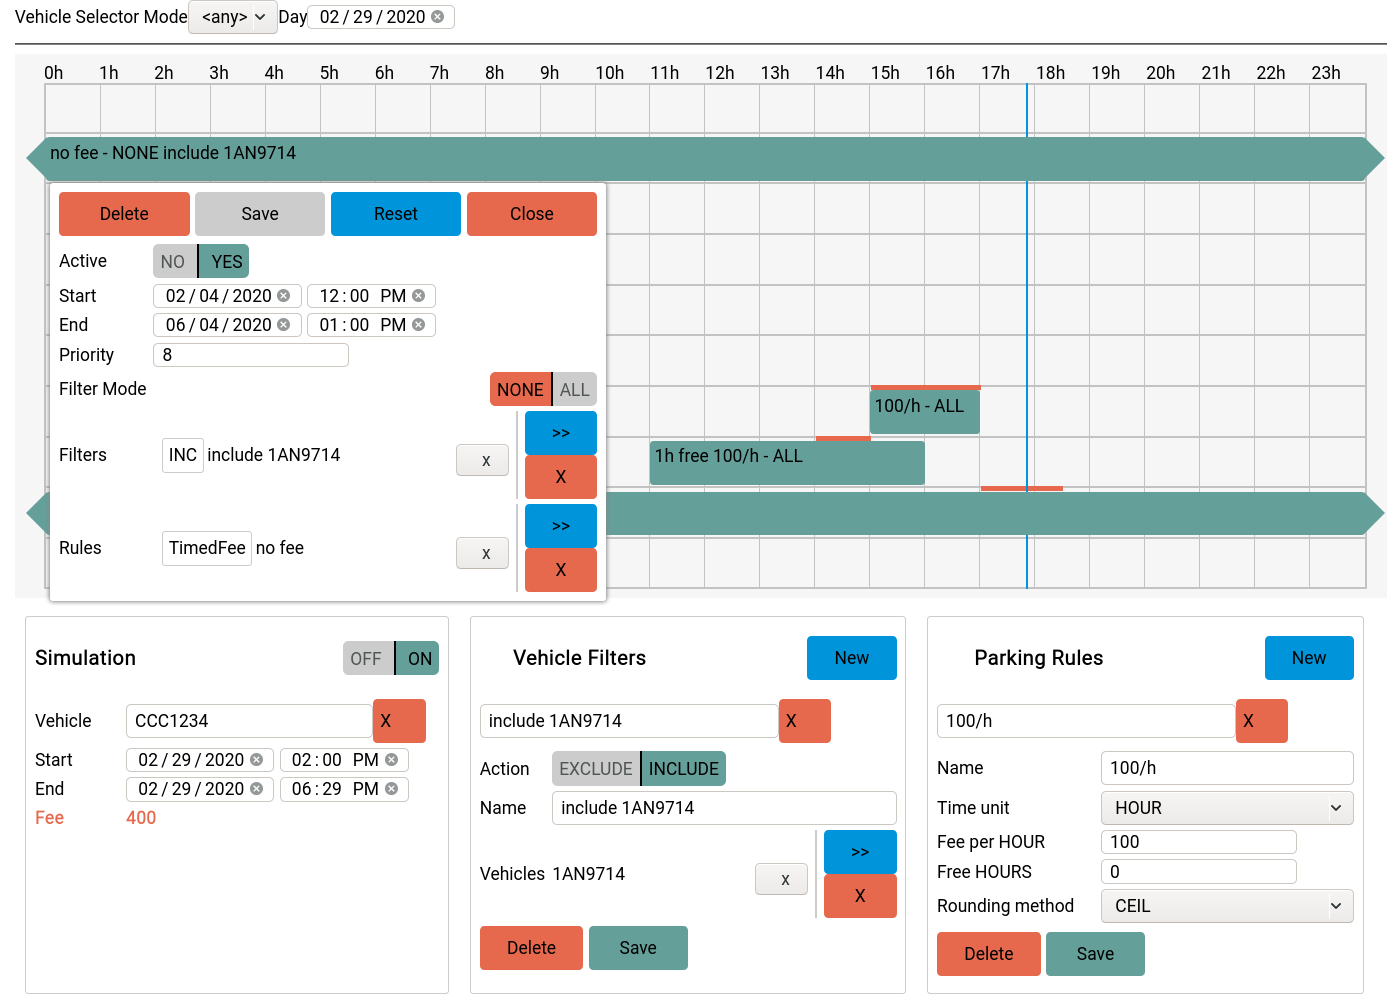
\includegraphics[width=145mm]{../img/page_rules.png}
  \caption{Stránka s pravidly, filtry a simulací pravidel.}
  \label{fig:page_rules}
\end{figure}

Viz obrázek \ref{fig:page_rules}.
Oranžová linka v kalendáři značí simulaci pravidel, jejíž výsledek je cena viditelná vlevo
dole v sekci Simulation.

\subsection*{Vozidla a parkování}

\begin{figure}[!htb] \centering
  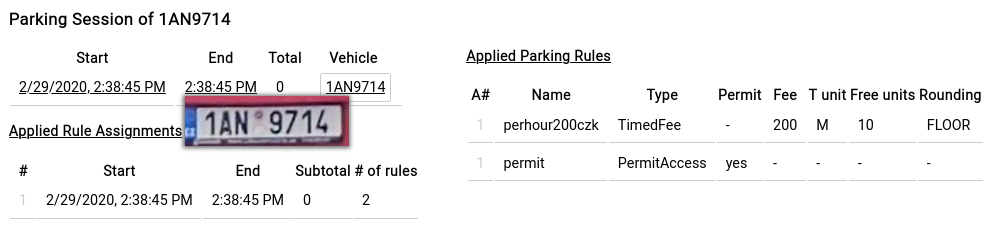
\includegraphics[width=145mm]{../img/page_vehicles1.png}
  \caption{Záznam o parkování.}
  \label{fig:page_session}
\end{figure}

Viz obrázek \ref{fig:page_session}.
Pokud uživatel najede myší na čas vjezdu nebo výjezdu, tak se mu zobrazí výřez SPZ z pořízeného snímku.
Zároveň lze kliknout na SPZ a zobrazit si ostatní záznamy onoho vozidla na stejné obrazovce.
Součástí záznamu je i kopie použitých pravidel, protože mohou být zpětně změněna správcem.
